\documentclass[12pt, letterpaper]{article}
\usepackage{polyglossia}
\usepackage{graphicx}
\usepackage{pdfpages}

\setmainlanguage{english}
\setotherlanguage{arabic}

\newfontfamily\arabicfont[Script=Arabic,Scale=1.5]{Scheherazade}

\title{\Huge\center{The Punt Reliefs and Their Significance on Hatshepsut's Reign}

\Large\scshape{Ancient History}}
\author{Samim Khaleqi}
\date{\today}
\begin{document}

\maketitle

\pagebreak
\tableofcontents
\pagebreak

\section*{Introduction}
\addcontentsline{toc}{section}{Introduction}
Ancient Egyptian society brings many thoughts to mind, such as pyramids, old mummified pharaohs, and even aliens.⸮ This ancient society, situated on the Nile River, has been flourishing from 3150 BC to 30 BC, and its impacts are still visible today.

One of ancient Egypt's most remarkable female pharaohs, Hatshepsut (1479–1458 BC), ruled during the New Kingdom of Egypt (1549–1077 BC) (Wicker, 1998, p. 155). Her reign saw the ambitious building projects from her prosperous economic performance, thanks to the emphasis on trading with neighbouring lands rather than military conquest. One of the more significant trade expeditions she conducted was to the land of Punt (modern-day Somalia), which is depicted in her mortuary temple in Deir el-Bahri\footnote{Dier el-Bahri is the transliteration of its Arabic name, ‘\textarabic{الدير البحري} ’ which translates to “The Northern Monastery.”} as the Punt expedition reliefs.

Though these sources provide us with valuable information for understanding how Hatshepsut had implemented her foreign policy and self- \\ representation as the divine ruler of Egypt, they may have certain biases due to the nature and propaganda of the time, which will be discussed later on.

\newpage
\begin{figure}
    \centering
    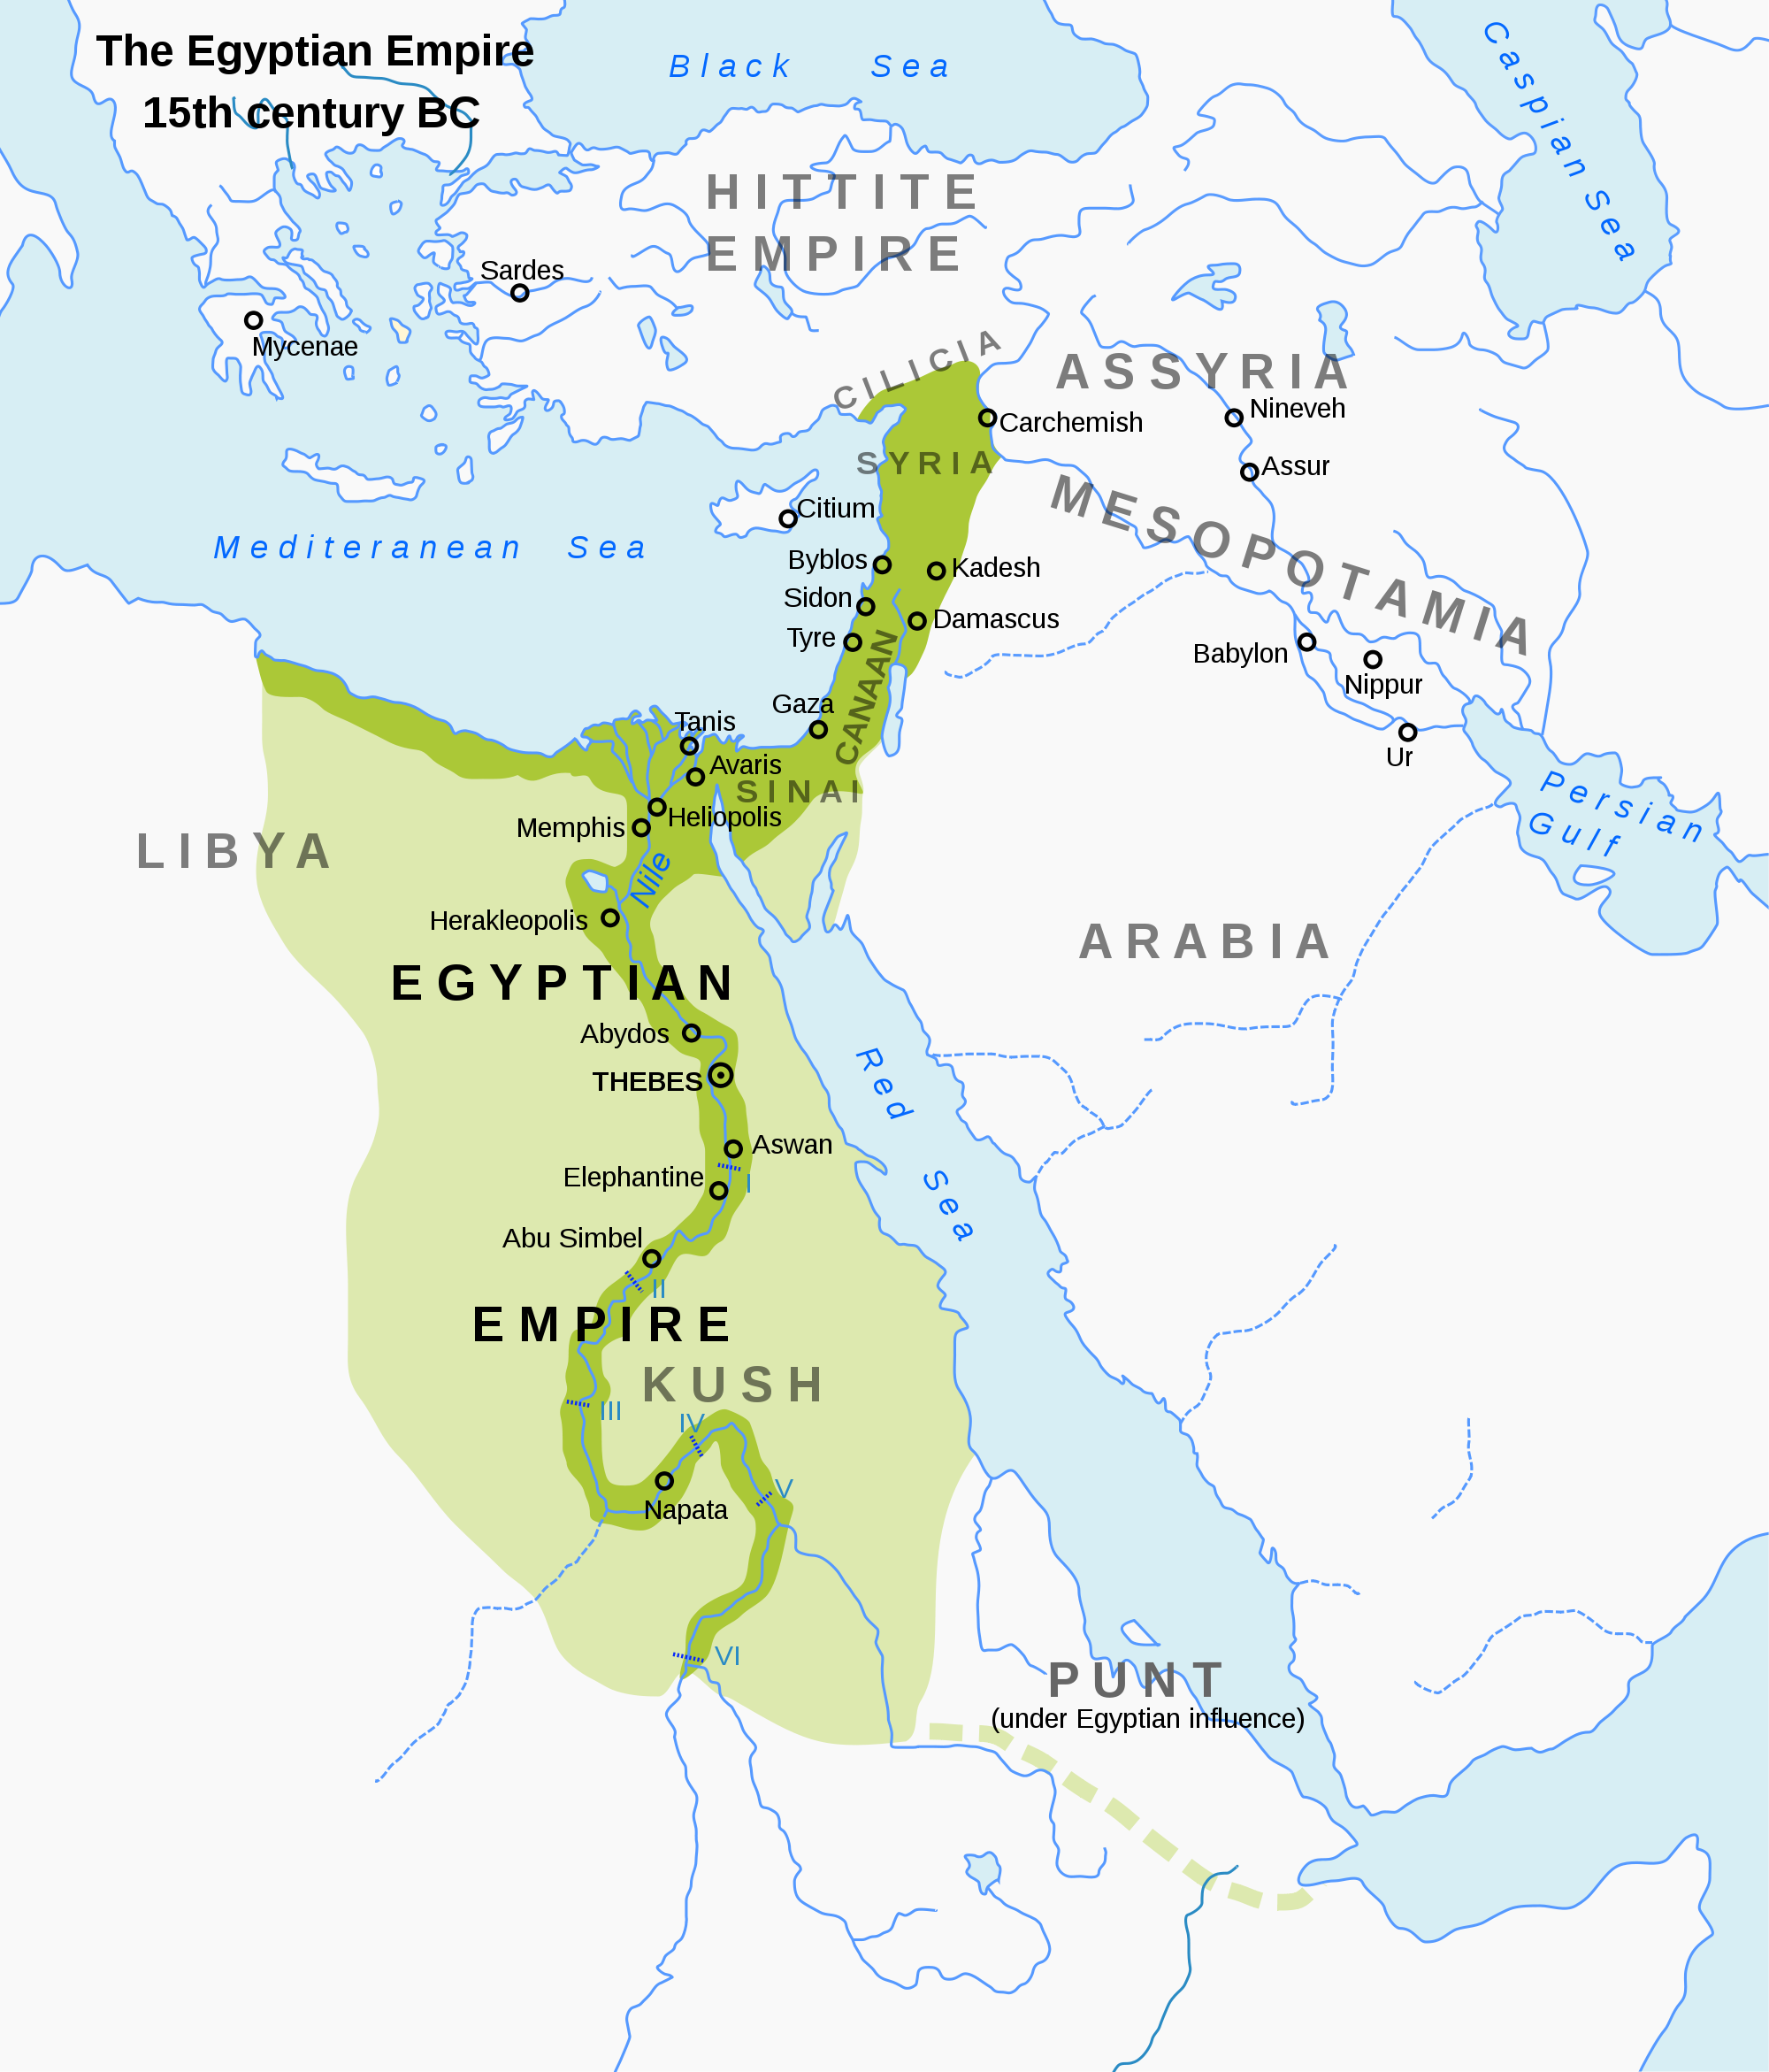
\includegraphics[width=0.8\linewidth]{img/map1.png}
    \caption{Map of Ancient Egypt approximately when Hatshepsut was in power.}
    \label{fig:enter-label}
\end{figure}


\section*{What are the Punt Reliefs?}
\addcontentsline{toc}{section}{What are the Punt Reliefs?}
The Punt expeditions were a significant part of Hatshepsut's reign, as they allowed her to demonstrate her diplomacy and economic skills rather than use a military conquest. Punt was originally called “The Land of the Gods,” and this provided luxury exotic goods such as ebony, incense, myrrh trees, ivory, gold, aromatic woods such as cinnamon, animal skins, etc. \footnote{American Research Centre in Egypt, 2007}, which were later used by priests in temple rituals to the gods. The importation of these materials reinforced the idea that Hatshepsut was a ruler who cared for the stability of the land.

Dier el-Bahri had become a part of Hatshepsut's building programme, where it would serve as not only a historical site but also a propaganda tool. Where the temple at first was dedicated to Amun, chief god of Thebes, built later to include her Punt Expeditions into her mortuary temple, Hatshepsut could reinforce her divine connection to the gods by portraying Amun as support for the expedition, legitimising her rule, showing that she was more than capable of being pharaoh since divine sanction strengthened her position even more.

Not only did the expedition of these goods provide Egyptian priests with important incense and sacrificial offerings that boosted and bolstered the economy, but it also allowed Hatshepsut to use it as a propaganda tool, as Amun is seen acknowledging her efforts, implying that the expedition was not only just for the economy but also to fulfil a divine will from the gods, not only legitimising but also normalising her rule over Egypt.


\section*{Relation To Her Foreign Policy}
\addcontentsline{toc}{section}{Relation To Her Foreign Policy}
The Punt Expedition reliefs are linked to Hatshepsut's foreign policy dot point especially about her military campaigns to expedition to Punt (ACHAH246). These records were a significant achievement for Hatshepsut's reign and provide a detailed account of her expedition, but unlike previous rulers, Hatshepsut did not focus on conquering the land of Punt, but rather she chose to strategically use it as a trade and diplomacy hub for her foreign policy \footnote{Tyldesley 1998.}.

The reliefs located at her mortuary temple at Deir el-Bahri are shown to illustrate the religious and ideological image of Hatshepsut's foreign policy. This is due to the expedition not solely being based on economical reasons but rather starting out as a religious mission like modern Mormon missionaries seen today \footnote{Dell, 2009.}. This religious expedition was started initially by Egyptian god Amun, where the reliefs can be seen depicting Hatshepsut receiving divine order for this mission, helping her own image as a ruler divinely chosen by the gods \footnote{Dell, 2009} \footnote{Tyldesley, 1998}. By choosing this inclusion in her reliefs, Hatshepsut could justify her role as a female pharaoh, so this connection between her foreign policy and divine religious ideology provides us with a key aspect to understanding how Hatshepsut had so much power at the time \footnote{Hillard, Wurtzel, 2009}.

However, it must be noted that this must be analysed due to the propagandistic flaws of these reliefs. Hatshepsut had likely exaggerated the events that took place to make her own image seem stronger, and there seem to be no difficulties or hardships in any of her Punt reliefs, making it difficult to give a true story of events. Another limitation is the defacement of the reliefs by her stepson Thutmose III, which raises the question, “Why?” Was Thutmose III jealous of his stepmother and wanted himself to be the main royal image? It's difficult to answer this due to historical inaccuracies, but Egyptologist Peter Doorman \footnote{The University of Chicago, 2025} noted that “For some reason, Thutmose III must have decided it was necessary to essentially rewrite the official record of Hatshepsut's kingship." (Wilson, 2006) This provides information about the situation: Thutmose III wanted all traces of Hatshepsut destroyed to write a new royal story for himself.

\begin{figure}
    \centering
    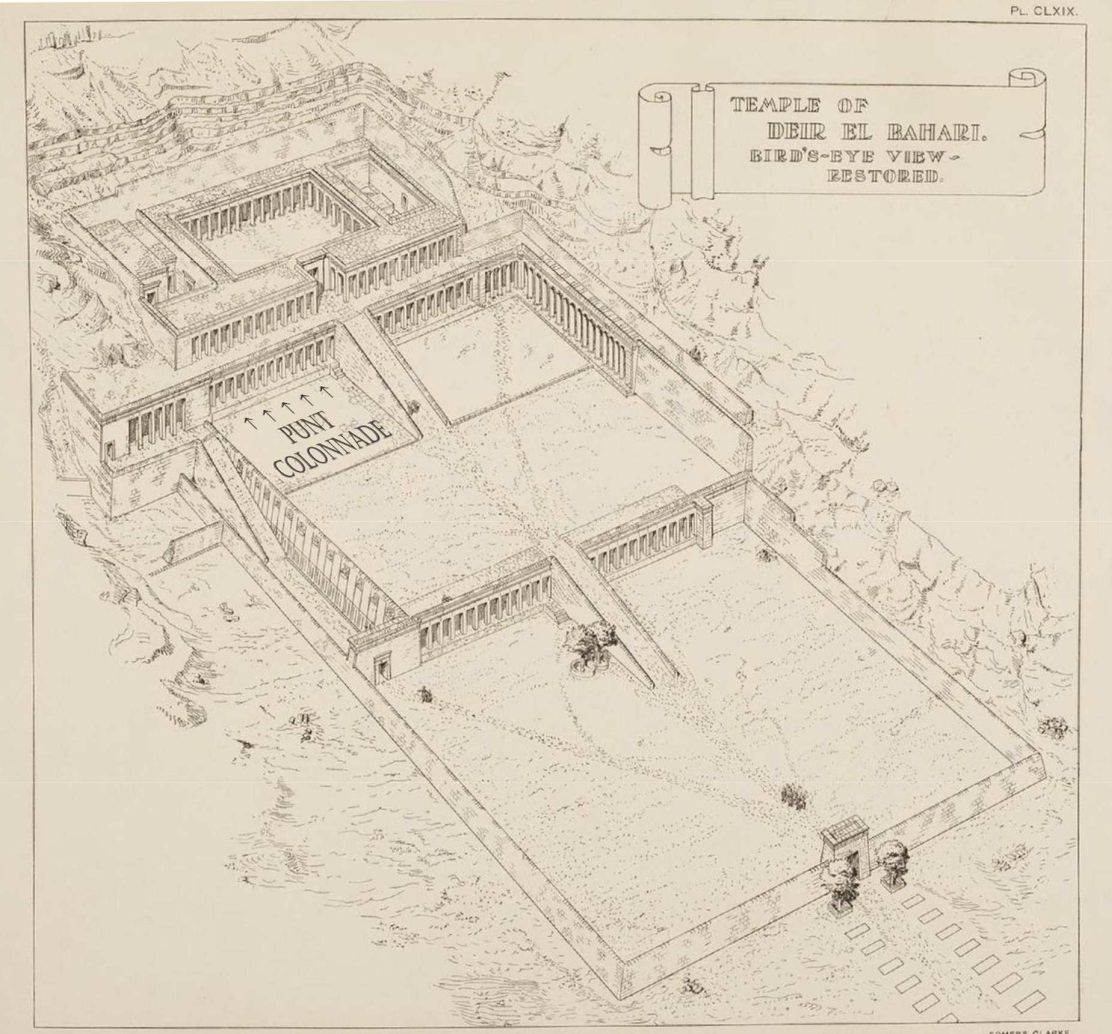
\includegraphics[width=1\linewidth]{img/map2.png}
    \caption{Map of Hatshepsut's Mortuary temple}
    \label{fig:enter-label}
\end{figure}
\newpage

\section*{An OPVL analysis of the Reliefs}
\addcontentsline{toc}{section}{An OPVL analysis of the Reliefs}
Hatshepsut's Punt Expedition reliefs serve as a valuable source of information, and they help us to understand what kind of power and capabilities she had during her reign, but it's important to check the facts and context of the reliefs using OPVL\footnote{OPVL is a technique used by the International Baccalaureate (IB), a non-profit international education organisation (International Baccalaureate Organisation, 2013). It helps to analyse and critically observe historical documents or historical pieces. OPVL stands for Origin. Purpose. Value. And Limitations. In order to analyse a source, you must know its origins; the more that is known about a piece of a source will help determine its purpose, value, and limitations. (Du, 2021) (IB History of the Americas, 2009)}.

\subsection*{Origin}
\addcontentsline{toc}{subsection}{Origin}
These reliefs were created during the time of Hatshepsut's reign at her mortuary temple, and it's possible that Hatshepsut's close advisor, Senenmut, to whom she had a suspected romantic relationship \footnote{(Hinds, 2007, p.27)}. This is significant because it signifies that Hatshepsut wanted to show her efforts as a pharaoh and promote her achievements, but Hatshepsut having commissioned the Punt reliefs causes potential bias, as they can be used to her benefit to show a particular political agenda.

\subsection*{Purpose}
\addcontentsline{toc}{subsection}{Purpose}
The purpose of the relief serves a multitude of purposes, from initially being a tool to glorify Hatshepsut as the new pharaoh to her being able to peacefully conduct expeditions to bring wealth and prosperity to Egypt. Though as much as Hatshepsut liked to glorify herself, these reliefs also show her divine bloodline and connection to Amun, who is seen in these reliefs sanctioning the expedition (FIG X). The connection to Amun helps her push her image in a male-dominated society at the time, helping her gain public notoriety.

\subsection*{Value}
\addcontentsline{toc}{subsection}{Value}
These reliefs were used in this assignment to create a model of the reliefs themselves, due to them being the most well-documented and dedicated trade missions in ancient Egyptian history. The evidence for this event even occurring is located in the residue of myrrh being located all around Egyptian religious sites; even though myrrh is not native to Egypt, this supports the claim that goods were brought back from Punt. Additionally, there are Egyptian texts from after Hatshepsut's reign that confirm Punt as a trading partner, confirming that Hatshepsut had established this trade route \footnote{Bunson, 2012, p.161}.

\subsection*{Limitations}
\addcontentsline{toc}{subsection}{Limitations}
However, it must be noted that even though we want to accept these Punt reliefs at face value, the propagandist nature of them cannot be ignored. These reliefs only really show an idealistic version of how the events really went down, as discussed in the last section. These fail to show any difficulty or hardship in acquiring the goods from Punt, and due to this context, clues may need to be used to show a true image of the journey rather than a divine Amun-sanctioned expedition to glorify Hatshepsut.


\section*{Conclusion}
\addcontentsline{toc}{section}{Conclusion}
The Punt Expedition Reliefs in her mortuary temple at Deir el-Bahri show the extraordinary achievements of Hatshepsut, from going to suspected lands that haven’t been visited in over 400 years and providing her kingdom with valuable resources such as incense and myrrh, gold, ivory, and exotic animals. This helped Hatshepsut showcase her rule in Egypt by completing successful trade deals and her preference for peaceful trade over large military conquests that would lead to mass casualty. This also strengthened Egypt’s economy during this time, showing her role as a leader and a provider for her people.

It shows just how much of a testament these foreign policies were to Hatshepsut to legitimise her rule as a female pharaoh. Her ingenuity and ambition showcase her divine favour, which further helped shape the view of her public image. After analysing the source of these reliefs, it can be concluded that even though there are themes of propaganda included within these murals, it still is a valuable source of information that can be backed up by future historians and evidence of her expenditure. By using all this information, it can be concluded that this provides a deep understanding of how Hatshepsut's reign had an impact on New Kingdom foreign policy, cementing her as one of the great female pharaohs.


\pagebreak
\includepdf[page=28]{img/mort.pdf}
\begin{figure}
    \centering
    \caption{Digital Collage Reconstruction of the Punt Reliefs at Hatshepsut's Mortuary temple (Docter and Thomas, 2012).}
    \label{fig:enter-label}
\end{figure}

\begin{figure}
    \centering
    \includegraphics[width=0.8\linewidth]{img/IMG_20250203_195303_129.jpg}
    \caption{My recreation of the Punt Relief's. Made out of a piece of tabletop wood, engraved with a dremel tool, epoxy filled, sanded, and finally clear coated.}
    \label{fig:enter-label}
\end{figure}
\newpage

% Referencing
\section*{\huge\textbf{References}}
\addcontentsline{toc}{section}{References}

American Research Center in Egypt (2007). Journal of the American Research Center in
Egypt. American Research Center in Egypt. Volumes 41-43. \\

Bunson, M. (2012). Encyclopedia of ancient Egypt. New York: Facts On File, p.161.
Dell, P. (2009). Hatshepsut : Egypt’s first female pharaoh. Minneapolis, Minn.: Compass Point Books. \\

Docter , R. and Thomas, V.D. (2012). Discourse on the Historical and Contemporary
Importance of Queen Hatshepsut’s Punt Expedition. [online] Available at: 

https://
www.academia.edu/download/59201276/
Queen\_Hatshepsuts\\ \_Punt\_Expedition\_FINAL\_online\_version20190510-90748-
kzu439.pdf. \\

Du, R. (2021). Keystone Academy Libraries: OPVL: What is OPVL? [online]
keystoneacademy-cn.libguides.com. Available at: \\ https://keystoneacademy-
cn.libguides.com/opvl. \\

Hinds, K. (2007). The Pharaoh’s Court. New York: Marshall Cavendish Benchmark, p.27.
IB History of the Americas (2009). A Guide to Origin, Purpose, Value and Limitations
(OPVL) IB History of the Americas Name. [online] Available at: https://
coulombesclass.wordpress.com/wp-content/uploads/2009/08/a-guide-to-opvls.pdf. \\

International Baccalaureate Organization (2013). Overview of the International
Baccalaureate. [online] Archive.org. Available at: \\ https://web.archive.org/
web/20141122173303/http://www.ibo.org/who/. \\

Kristina Hilliard \& Kate Wurtzel (2009) Power and Gender in Ancient Egypt: The Case of Hatshepsut, Art Education, 62:3, 25-31. \\

The University of Chicago (2025). Peter Dorman | Middle Eastern Studies. [online]
Uchicago.edu. Available at: https://mes.uchicago.edu/people/peter-dorman [Accessed 4
Feb. 2025]. \\

Tyldesley, J.A. (1998). Hatchepsut : the female pharaoh. London: Penguin.
Wicker, F.D.P. (1998). The Road to Punt. The Geographical Journal, 164(2), pp.155–167. doi:https://doi.org/10.2307/3060367. \\

Wilson, E.B. (2006). The Queen Who Would Be King. [online] Smithsonian. Available at:
https://www.smithsonianmag.com/history/the-queen-who-would-be-king-130328511/.


\end{document}
